\chapter{背景介绍}
本章中简要介绍本文工作中的一些重要的基础知识。本章将分为三节。第一节介绍量子计算相关背景,包括量子力学和量子线路。第二节介绍模型检测相关背景,包括跃迁系统,时序逻辑和量子模型检测。第三节介绍TDD相关背景,包含TDD的定义和与类似方法的比较。
\section{量子计算简介}
本节将简单介绍量子计算相关的背景内容,具体内容可以参考
\citep{nielsen2010quantum}。
本节将分两个部分介绍量子计算相关背景,第一部分介绍量子力学,第二部分介绍量子线路模型。

量子计算机(quantum computer)是一种利用量子比特特性进行计算的一种设备。
而量子力学就是描述量子比特特性的理论。
量子比特的特殊性质在于其可以同时处于多种状态,这与经典比特的二进制状态不同。量子比特的状态空间可以用希尔伯特空间(Hilbert space)\(\mathcal{H}\)表示\citep{nielsen2010quantum},即可以进行内积运算(inner product)的复向量空间。因此比特状态可以用\(\mathcal{H}\)的向量表示,量子操作用\(\mathcal{H}\)上的线性算子(linear operator)表示。

而量子线路(quantum circuit)是一种描述量子计算的模型\citep{nielsen2010quantum}。在量子线路中,通过量子比特的初始化、应用量子门、测量以及其他可能的操作的序列来构建和执行量子计算任务。量子线路通常从左向右阅读,每个量子门的作用是将输入的量子比特状态转变为输出状态,该过程可以认为是量子门的酉矩阵与输入的量子状态的乘积。
\begin{example}
    \label{ex-epr}
    图\ref{fig:example_cir} 所示的量子线路展示了一个具体的量子线路示例,可以用于制备EPR态。其中有单比特门\(H\),以及双比特门\(CX\)。假设该量子线路的初始状态为\(\left|\psi\right\rangle=\left|0\right\rangle\left|0\right\rangle\),则输出状态为:
\begin{align}
   \frac{|00\rangle+|11\rangle}{\sqrt{2}}
\end{align}
不同量子操作的含义将在\ref{sec-mat}节中具体介绍,关于该量子线路的具体计算过程将在\ref{sec-cir}节中介绍。
\end{example}
\begin{figure}[!htbp]
    \centering
    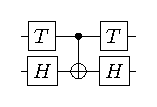
\includegraphics[width=.4\textwidth]{Img/example_cir.pdf}
    \caption{制备EPR态的量子线路图}
    \label{fig:example_cir}
\end{figure}



在量子计算机上可以执行各种算法和计算任务,如量子搜索\citep{Grover_1996}、量子因子分解\citep{Shor}和量子模拟\citep{Feynman}等。量子计算的潜力在于其能够在某些特定问题上比经典计算机更高效地进行计算,尤其在处理大规模数据和解决复杂问题方面具有潜在优势。

\subsection{量子力学}
量子力学有两种主要的表述:波动力学和矩阵力学。其中波动力学由Erwin Schrödinger首创,矩阵力学由Werner Heisenberg首创。波动力学使用微分方程为数学基础,更接近于经典物理的波动理论,适用于处理时间演化问题和连续系统。
而矩阵力学使用线性代数为数学基础,适用于具有离散能级的系统。由于在量子计算中,大量使用矩阵力学作为理论基础。
因此本小节主要介绍矩阵力学。
\subsubsection*{线性代数}
线性代数的基本研究对象是向量空间(vector space),也称作线性空间(Linear Spaces)。这是一种抽象的数学结构,用于描述向量的集合。向量空间在向量加法(Vector Addition)和标量乘法(scalar multiplication)封闭\cite{greub2012linear}。
对于一个向量空间,向量的类型满足特定条件。向量可以是几何向量、函数、多项式或任何满足向量空间公理的对象。
同时还需要定义标量域(Scalars)\(\mathbb{F}\) ,在大多数情况下,标量是实数(Real Numbers)\(\mathbb{R}\)或复数(Complex Numbers)\(\mathbb{C}\),用于通过标量乘法运算改变向量的大小。
最后向量空间的还需要遵循一系列公理。这些公理规定了向量加法和标量乘法的性质,如加法的交换律和结合律、加法和标量乘法的分配律、加法单位元的存在性(即零向量,Zero Vector),以及乘法单位元(即标量1)的存在性。这些公理确保了向量空间内运算的一致性和预测性。

此外子空间(Subspace)也是是向量空间中的一个重要概念。子空间指的是一个向量空间的一个子集,同时它自身也是一个向量空间。因此子空间遵循向量空间的向量加法和标量乘法运算封闭的性质。线性算子 (Linear Operator),也称为线性映射(Linear Mapping)或线性变换(Linear Transformation),是在向量空间中的一种特殊函数,它在两个向量空间之间映射向量,保持向量加法和标量乘法的结构。线性算子定义如定义\ref{def-op}所示。% 线性算子定义
\begin{definition}\citep{greub2012linear}
    \label{def-op}
    设 \(V\) 和 \(W\) 是两个向量空间,算子 \(T: V \rightarrow W\) 是线性算子,当且仅当\(T\)满足以下两个条件:
\begin{enumerate}
    \item 加法性 (Additivity):对于所有 \(u, v \in V\),有 \(T(u + v) = T(u) + T(v)\)。
    \item 齐次性 (Homogeneity):对于所有标量 \(a \in \mathbb{F}\) 和所有 \(v \in V\),有 \(T(av) = aT(v)\)。
\end{enumerate}
\end{definition}

当$T$是\(T: V \rightarrow V\)的线性算子,则称$T$是定义在向量空间$V$上的线性算子。其中恒等算子(identity operator)是一类特殊的线性算子,其定义如定义\ref{def-id}所示。
\begin{definition}\citep{greub2012linear}
    \label{def-id}
    设 \(V\) 是一个向量空间,$T$是向量空间$V$上的线性算子。$T$是恒等算子,当且仅当$T$满足以下条件:
    \begin{align}
        T(v) = v,\quad \forall v \in V
    \end{align}
\end{definition}

此外有的向量空间还有内积(inner product)和张量积(tensor product)操作。而内积定义如定义\ref{def-pro}所示。
\begin{definition}\citep{greub2012linear}
    \label{def-pro}
    设 \(V\) 是一个向量空间,
    \(V\)上有一个映射\(( \cdot, \cdot ): V \times V \rightarrow \mathbb{F}\)。该映射是内积,当且仅当对于任意两个向量 $u$ 和 $v$, $( u, v )$ 满足以下性质:
\begin{enumerate}
    \item 共轭对称性(Conjugate Symmetry): \(( u, v ) = \overline{( v, u )}\),其中\(\overline{( v, u )}\)是\(( v, u )\)的复共轭,当标量域为实数时,表现为对称性,即\(( u, v ) = ( v, u )\)。
    \item 线性 (Linearity)或齐次性:\(( \alpha u_1 + \beta u_2, v ) = \alpha( u_1, v ) + \beta( u_2, v )\),其中\(\alpha,\beta\in\mathbb{F}\)。
    \item 正定性 (Positive Definiteness):\(( v, v ) \geq 0\)且仅当\(v \)为加法单位元时等号成立。
\end{enumerate}
\end{definition}
% 张量积定义
可以看到内积是一种特殊形式的线性算子。当两个向量内积为$0$时,称这两个向量正交。而张量积则提供了一种方法来构造新的向量空间。其定义如定义\ref{def-tensor-product}所示。
\begin{definition}\citep{greub2012linear}
    \label{def-tensor-product}
    设 \(V\) 和 \(W\) 是两个向量空间,它们的张量积 \(V \otimes W\) 是一个新的向量空间,其必须满足以下性质:
\begin{enumerate}
    \item 对于每一对元素 \(v \in V\) 和 \(w \in W\),存在一个元素 \(v \otimes w \in V \otimes W\),称为它们的张量积。
    \item 张量积满足双线性性(Bilinearity):对于所有 \(v,v' \in V\),\(w,w' \in W\) 以及所有标量 \(a,b \in \mathbb{F}\),有
    \begin{align}
    (av + bv') \otimes w = a(v \otimes w) + b(v' \otimes w),\\
    v \otimes (aw + bw') = a(v \otimes w) + b(v \otimes w').
    \end{align}
    \item 张量积是唯一的,意味着对于任何与 \(V \otimes W\) 具有相同性质的向量空间,都存在一个自然同构映射(Natural Isomorphism)到 \(V \otimes W\)。
\end{enumerate}
\end{definition}


矩阵力学的数学基础建立在希尔伯特空间\(\mathcal{H}\),即一个可以进行内积运算的复向量空间。
希尔伯特空间中的向量由复数\(n\)元组\(\left(c_1,c_2,\cdots,c_n\right)\)构成,可以记作\(\mathbb{C}^n\),其中\(c\)表示复数。因此复向量也可以有以下列矩阵形式:
\begin{align}
    \left[\begin{matrix}
        c_1\\c_2\\\vdots\\c_n
    \end{matrix}\right]
\end{align}
\(\mathbb{C}^n\)中的标量为复数。因此可以定义\(\mathbb{C}^n\)矩阵形式的标量乘法运算为:
\begin{align}
    c'\left[\begin{matrix}
        c_1\\c_2\\\vdots\\c_n
    \end{matrix}\right]=\left[\begin{matrix}
        c'\cdot c_1\\c'\cdot c_2\\\vdots\\c'\cdot c_n
    \end{matrix}\right]
\end{align}
其中等式右边的乘法为复数乘法,因此复数1为乘法单位元。类似地,\(\mathbb{C}^n\)矩阵形式的向量加法可以定义为:
\begin{align}
    \left[\begin{matrix}
        c_1\\c_2\\\vdots\\c_n
    \end{matrix}\right]
    +\left[\begin{matrix}
        c'_1\\c'_2\\\vdots\\c'_n
    \end{matrix}\right]=\left[\begin{matrix}
        c_1+c'_1\\c_2+c'_2\\\vdots\\c_n+c'_n
    \end{matrix}\right]
\end{align}
其中等式右边的乘法为复数加法,因此零向量的矩阵形式如下:
\begin{align}
    \left[\begin{matrix}
        0\\0\\\vdots\\0
    \end{matrix}\right]
\end{align}
通常将该向量记作\(\mathbf{0}\)。

类似地,可以定义\(\mathbb{C}^n\)矩阵形式的内积和张量积运算为:
\begin{align}
    \left(\left[\begin{matrix}
        c_1\\c_2\\\vdots\\c_n
    \end{matrix}\right]
    ,\left[\begin{matrix}
        c'_1\\c'_2\\\vdots\\c'_n
    \end{matrix}\right]\right)=
    \sum_{i=1}^{n}c_i^* c'_i
\end{align}
\begin{align}
    \left[\begin{matrix}
        c_1\\c_2\\\vdots\\c_n
    \end{matrix}\right]
    \otimes\left[\begin{matrix}
        c'_1\\c'_2\\\vdots\\c'_n
    \end{matrix}\right]=\left[\begin{matrix}
        c_1c'_1\\c_1c'_2\\\vdots\\c_1c'_n\\c_2c'_1\\\vdots\\c_n c'_n
    \end{matrix}\right]
\end{align}
在量子计算中,通常将向量\(\psi\)记作狄拉克右矢符号\(|\psi\rangle\)。
对向量\(|\psi\rangle\)中的复数全部取共轭,可以得到\(|\psi\rangle\)的共轭记作\(|\psi\rangle^*\)。
向量\(|\psi\rangle\)的共轭转置可以记作\(|\psi\rangle^\dagger\),也称对偶向量,可以用狄拉克左矢符号\(\langle\psi|\)表示。因此向量之间的内积也可以用以下方法表示:
\begin{align}
    (|\psi\rangle, |\phi\rangle)=\langle \psi|\phi\rangle ,\quad \forall |\psi \rangle, |\phi \rangle\in \mathcal{H}
\end{align}

希尔伯特空间\(\mathcal{H}\)中的线性算子集合,通常记作\(\mathcal{L} (\mathcal{H})\)。对于算子$A$,其伴随算子(adjoint operator)$A^\dagger$的定义如定义\ref{def-dagger}所示。
在伴随算子基础上可以如定义\ref{def-hermite}所示,定义Hermite算子(Hermite operator)。
\begin{definition}\citep{nielsen2010quantum}
    \label{def-dagger}
    设算子\(A \in \mathcal{L}(\mathcal{H})\),\(A^\dagger\)是$A$的伴随算子满足,那么\(A^\dagger\)满足:
\begin{align}
    \langle \psi |A^\dagger|\phi \rangle = \langle \phi |A|\psi \rangle^*,\quad \forall |\psi \rangle, |\phi \rangle\in \mathcal{H}
\end{align}
\end{definition}
\begin{definition}\citep{nielsen2010quantum}
    \label{def-hermite}
    设算子\(A \in \mathcal{L}(\mathcal{H})\)。算子\(A\)是Hermite算子,当且仅当\(A\)满足:
\begin{align}
    A = A^\dagger
\end{align}
\end{definition}


而在Hermite算子的基础上,可以继续定义几类重要的算子,如定义\ref{def-proj}中的投影算子(project oroperator),定义\ref{def-normal}中的正规算子(normal oroperator),以及定义\ref{def-unitary}中的酉算子(unitary oroperator)。
\begin{definition}\citep{nielsen2010quantum}
    \label{def-proj}
    设算子\(A \in \mathcal{L}(\mathcal{H})\),且\(A\)是Hermite算子。那么\(A\)是投影算子,当且仅当\(A\)满足:
\begin{align}
    A^2 = A
\end{align}
\end{definition}

\begin{definition}\citep{nielsen2010quantum}
    \label{def-normal}
    设算子\(A \in \mathcal{L}(\mathcal{H})\),且\(A\)是Hermite算子。那么\(A\)是正规算子,当且仅当\(A\)满足:
\begin{align}
    A^\dagger A = A A^\dagger
\end{align}
\end{definition}

\begin{definition}\citep{nielsen2010quantum}
    \label{def-unitary}
    设算子\(A \in \mathcal{L}(\mathcal{H})\),且\(A\)是Hermite算子。那么\(A\)是酉算子,当且仅当\(A\)满足:
\begin{align}
    A^\dagger A = I
\end{align}
其中$I$表示希尔伯特空间中的恒等算子。
\end{definition}

其中酉算子保持向量之间的内积,即:
\begin{equation}
    \begin{split}
        (U|\psi\rangle, U|\phi\rangle) &= \langle \psi|U^\dagger U|\phi\rangle \\
        &= \langle \psi|I|\phi\rangle = \langle \psi|\phi\rangle = (|\psi\rangle, |\phi\rangle), \forall |\psi \rangle,\quad |\phi \rangle\in \mathcal{H}
    \end{split}
\end{equation}
\subsubsection*{量子力学基本假设}
在量子力学中,有四条基本假设,其数学框架是在不断实验中总结,假设,验证而得到的。
下面分别简单介绍一下这四条假设。
\begin{theorem}\citep{nielsen2010quantum}
    每个孤立的物理系统都可以通过一个内积复向量空间(即希尔伯特空间)来表征,此空间被视为系统的状态空间(state space)。该系统的全部性质由位于状态空间内的一个单位向量,即状态向量(state vector),完整定义。
\end{theorem}

量子力学的第一条假设,提出了量子系统的描述方式。最简单的量子系统是单个量子比特(qubit)构成的二维空间。
取$|0\rangle$和$|1\rangle$为该状态空间的一组标准正交基,则该状态空间中的所有状态向量$|\psi\rangle$都可以用以下方式表示:
\begin{align}
    |\psi\rangle = \alpha|0\rangle + \beta|1\rangle
\end{align}
其中$\alpha,\beta\in \mathbb{C}$,并满足:
\begin{align}
    |\alpha|^2+|\beta|^2  = 1
    \label{eq-cal}
\end{align}
等式\ref{eq-cal}确保了$|\psi\rangle$的模长为1,即保证了$|\psi\rangle$是单位向量:
\begin{align}
    \langle\psi|\psi\rangle = 1
    \label{eq-norm}
\end{align}
等式\ref{eq-norm}称为状态向量的归一化条件(normalization condition)。
而\(\alpha,\beta\)也被称为对应基状态向量的振幅(amplitude)。
\begin{example}
    式子\ref{eq-entag}中的叠加态,处在$|0\rangle$状态的振幅为$\frac{1}{\sqrt{2}}$,处在$|1\rangle$状态的振幅为$-\frac{1}{\sqrt{2}}$。
\begin{align}
    \label{eq-entag}
    \frac{|0\rangle-|1\rangle}{\sqrt{2}}
\end{align}
\end{example}
\begin{theorem}\citep{nielsen2010quantum}
    一个封闭量子系统(closed quantum system)的演化(evolution)由酉变化(unitary operation)体现。具体来讲,系统在$t_1$时刻的状态$|\psi\rangle$与在$t_2$时刻的状态$|\psi'\rangle$之间,通过一个只与$t_1$和$t_2$两个时间点相关的酉操作符$U$连接:
    \begin{align}
        |\psi'\rangle = U|\psi\rangle
    \end{align}
\end{theorem}
酉变化可以用酉算子进行表示。对于酉算子$U$, 始终满足
\begin{align}
    U U^\dagger = I
\end{align}
这是因为这些演化都是可逆的。当令单个量子比特的状态空间的正交基$|0\rangle$和$|1\rangle$的矩阵形式为:
\begin{align}
    |0\rangle = \left[\begin{matrix}
        1\\0
    \end{matrix}\right],|1\rangle = \left[\begin{matrix}
        0\\1
    \end{matrix}\right]
\end{align}
\label{sec-mat}
可以得到常见单比特酉变化的矩阵形式,比如Pauli算子:
\begin{align}
    I = \left[\begin{matrix}
        1,0\\0,1
    \end{matrix}\right]
    \quad
    X = \left[\begin{matrix}
        0,1\\1,0
    \end{matrix}\right]
    \quad
    Y = \left[\begin{matrix}
        0,-i\\i,0
    \end{matrix}\right]
    \quad
    Z = \left[\begin{matrix}
        1,0\\0,-1
    \end{matrix}\right]
    \label{eq-pauli}
\end{align}
比如Hardmard算子和T门(也可以称为\(\pi/8\)门):
\begin{align}
    H = \frac{1}{\sqrt{2}}\left[\begin{matrix}
        1,1\\1,-1
    \end{matrix}\right]
    \label{eq-hardmard}
\end{align}
\begin{align}
    T = \left[\begin{matrix}
        1,&0\\0,&\exp(i\pi/4)
    \end{matrix}\right]
    \label{eq-t}
\end{align}

\begin{theorem}\citep{nielsen2010quantum}
    量子测量(quantum measurement) 可以通过一系列测量算子 (measurement operator) ${M_m}$ 刻画。这些算符作用于被测量系统的状态空间上。其中下标$m$
   对应实验中可能发生的测量结果。
\end{theorem}
由于测量结果的概率和为1,因此测量算子${M_m}$满足完备性,即:
\begin{align}
    \sum_m M_m\dagger M_m = I
\end{align}
假设测量前量子系统的状态为\(|\psi\rangle\),那么测量后得到结果m的概率为
\begin{align}
    p(m) = \langle\psi|M_m^\dagger M_m|\psi\rangle
\end{align}
测量后,系统的状态变为
\begin{align}
    |\psi'\rangle =  \frac{M_m|\psi\rangle}{\sqrt{p(m)}} = \frac{M_m|\psi\rangle}{\langle\psi|M_m^\dagger M_m|\psi\rangle}
\end{align}
\begin{theorem}\citep{nielsen2010quantum}
    复合系统(composite system) 的状态空间是其各个子空间的状态空间的
    张量积。如果复合系统从$1$到$n$的子系统,并且第$i$个系统的状态为$|\psi_i\rangle$。则复合系统的状态为\(|\psi_1\rangle\otimes|\psi_2\rangle\otimes\cdots\otimes |\psi_n\rangle\)。
    \label{th-com}
\end{theorem}
假设\ref{th-com}中的复合系统,假设了子系统之间的相互作用,并没有改变复合系统状态空间的结构。
此时的复合系统处于直积状态(product state)。例如两个处于\(|0\rangle\)状态的单量子组成的双量子比特的复合系统,可以有以下方式的表示:
\begin{align}
    |0\rangle\otimes|0\rangle=\left[\begin{matrix}
        1\\0
    \end{matrix}\right]\otimes\left[\begin{matrix}
        1\\0
    \end{matrix}\right] = \left[\begin{matrix}
        1\\0\\0\\0
    \end{matrix}\right]
\end{align}
类似地,可以得到\(\ket{01},\ket{10},\ket{11}\)的矩阵形式。从而可以得到双量子复合系统的操作。式子\ref{eq-cx}为双量子复合系统中常见的受控非门操作的矩阵形式。
\begin{align}
    \label{eq-cx}
    CX=\left[\begin{matrix}
        1 & 0 & 0 & 0\\
        0 & 1 & 0 & 0\\
        0 & 0 & 0 & 1\\
        0 & 0 & 1 & 0\\
    \end{matrix}\right]
\end{align}


此外还存在复合系统的量子状态不能分解成各个子系统量子状态的张量积的情况。此时复合系统处于纠缠状态(entangled state),复合系统不能表示为子系统的张量积形式。
例如该双量子比特的复合系统的状态,就不能表示为任何单比特状态向量的张量积:
\begin{align}
    \frac{|00\rangle+|11\rangle}{\sqrt{2}}
\end{align}
\subsection{量子线路}
\label{sec-cir}
在经典计算机理论中,通常使用图灵机作为抽象模型。
在讨论图灵机时,会设想一个容量无限的计算机。然而在实际中,计算机的容量是有限的。
因此在实际讨论时,一般会使用线路模型,作为图灵机的替代模型。该模型在计算力方面与图灵机等价,但在许多应用场景中更为实用和符合实际。线路模型是由导线(wire)和逻辑门(gate)构成,它们分别负责信息的传递和基本计算操作。
\begin{example}
    图\ref{fig-not}展示了一个简单的经典线路。它以单个比特作为输入。这个比特通过一个门,该门会翻转比特,将1变为0,将0变为1。门前后的导线仅用于将比特信息传输到非门并从非门传出。
\begin{figure}[htbp]
    \centering
    \includegraphics[width=.3\textwidth]{Img/Not-gate-en}
    \caption{执行单个非门的经典基本线路}
    \label{fig-not}
\end{figure}
\end{example}

在量子计算类似,一般使用量子线路(quantum curcuit) 作为抽象模型。
在量子线路中,逻辑门为量子操作,导线则传递量子比特信息。量子操作可以由量子门(quantum gate) 表示。
根据量子门作用的量子比特数,量子门可以被分为单量子比特门(single qubite gate)和多量子比特门(multiple qubit gate)。多量子比特门中比较常见的是双量子比特门。
以受控门(controlled gate)为例,其
输入量子比特分别为控制量子比特(control qubit)和目标量子比特(target qubit)。
假设$U $是作用于目标量子比特的任意单比特量子操作,则称该门为受控$U$门。
受控$U$门根据控制量子比特的值,决定是否将量子操作$U$作用于目标量子比特。
若控制量子比特的值为\(|0\rangle\),则目标量子比特值\(|\psi\rangle\)不变,若控制量子比特的值为
\(|1\rangle\), 则目标量子比特值变为\(U|\psi\rangle\)。

而和经典线路模型不同,量子线路一般会固定阅读方向。量子信息固定从左到右传递。因此量子线路模型也可以看作经过一系列量子门,将线路左边的输入量子状态转换为线路右边的输出量子状态的模型。
综上通过量子线路可以描述各种量子计算的过程。
% //TODO: add more
\begin{example}
    单量子比特门Hadamard门为例,其矩阵形式为式子\ref{eq-hardmard}。因此其将输入的\(|0\rangle\)状态变换为
\(\frac{|0\rangle+|1\rangle}{\sqrt{2}}\)状态,\(|1\rangle\)状态变换为\(\frac{|0\rangle-|1\rangle}{\sqrt{2}}\)状态。其量子线路符号表示如图\ref{fig-h}所示。
\begin{figure}[htbp]
    \centering
    \includegraphics[width=.3\textwidth]{Img/hardmard-gate.pdf}
    \caption{Hadamard门的量子线路符号}
    \label{fig-h}
\end{figure}

    而受控门中最常见的是受控非门(controlled not gate),其矩阵形式为式子\ref{eq-cx}。若控制量子比特为\(|0\rangle\)则不做变换;若为\(|1\rangle\)则对目标量子比特进行比特翻转,将
输入的\(|0\rangle\)变换为\(|1\rangle\),\(|1\rangle\)变换为\(|0\rangle\)。其量子线路符号如图\ref{fig-cx}。
\begin{figure}[htbp]
    \centering
    \includegraphics[width=.3\textwidth]{Img/cnot-gate.pdf}
    \caption{受控非门的量子线路符号}
    \label{fig-cx}
\end{figure}

综上,例子\ref{ex-epr}中,包含一个Hadamard门和一个受控非门的制备EPR态的量子线路。当输入态为\(|00\rangle\)时,输出态为\(\frac{|00\rangle+|11\rangle}{\sqrt{2}}\)。具体计算过程如式子\ref{eq-eqr-cal}所示。
\begin{equation}
    \label{eq-eqr-cal}
    \begin{aligned}
        |\psi_{out}\rangle &=  CX\cdot H\otimes I \cdot \left|\psi_{in}\right\rangle\\
        &= CX\cdot H\otimes I \cdot \left|00\right\rangle\\
        &= CX\cdot H\otimes I \cdot \left|0\right\rangle\otimes \left|0\right\rangle\\
        &= CX\cdot H\left|0\right\rangle\otimes I\left|0\right\rangle\\
        &= CX\cdot \frac{|0\rangle+|1\rangle}{\sqrt{2}} \otimes\left|0\right\rangle\\
        &= \frac{|0\rangle|0\rangle+|1\rangle\otimes X|0\rangle}{\sqrt{2}}\\
        &=\frac{|00\rangle+|11\rangle}{\sqrt{2}}
    \end{aligned}
\end{equation}
\end{example}
\section{模型检测简介}
本节将简要介绍了模型检测中的跃迁系统、时序逻辑的验证以及量子模型检测。跃迁系统是模型检测的基础,定义了系统状态、行为及状态转移关系。时序逻辑用于指定待验证的属性,包括状态命题和路径命题。而量子模型检测利用Birkhoff-von Neumann量子逻辑描述量子系统的性质,展示了量子逻辑中命题的表示和逻辑结构。这些都为本文工作的研究提供了重要的理论基础。
\subsection{跃迁系统}
\label{sec-transition}
跃迁系统广泛应用于模型检测中待检测系统的建模,具体定义如定义\ref{def-model}所示。
\begin{definition}\citep{baier2008principles}
    \label{def-model}
    迁移系统为一个四元组,具体包含:
    \begin{equation}
        \mathcal{M}=(S, S_0, \Sigma, R)
    \end{equation}
    其中\(S\)为系统状态集合;\(S_0\)为系统初态集合,因此满足\(S_0\subseteq S\); $\Sigma=\{\sigma_1,\ldots,\sigma_m\}$ 表示符号的集合; $R \subseteq S \times \Sigma \times S$ 则代表转移关系。
\end{definition}

此外迁移系统还需要有\(AP\)描述系统原子命题。$L$是标记函数,将状态映射为状态满足的原子命题集合。需要验证的属性\(\varphi\)将表述为命题。对于某个状态集 $S' \subseteq S$,通过转移关系 $R$ 得到的系统状态可以表示为
\begin{equation}\label{eq:image}
R(S') := \{ t\in S \mid (s, \sigma, t) \in R\ \text{并且}\ s \in S', \sigma \in \Sigma\}
\end{equation}


系统的有限路径片段\(\pi\)是一个有限状态序列\(s_0,s_1\ldots s_n\),其中\(s_0\in S_0\)。\(s_i\)满足\(s_{i-1}\overset{\sigma_i}{\rightarrow}s_i,\sigma_i\in \Sigma\),对于所有\(0<i\leq n\),其中\(n\geq 0 \)。无限路径片段\(\pi\)是一个无限状态序列\(s_0,s_1\ldots\),使得对于所有\(i>0\),\(s_{i-1} \overset{\sigma_i}{\rightarrow}  s_i,\sigma_i\in \Sigma\)。在路径中\(\pi\left[i\right]=s_i,\pi\left[i\right)=s_i\ldots\)。所有以\(S_0\)为开始的路径,构成了路径集合\(Path\left(S_0\right)\)。

量子模型检测的跃迁系统类似。区别在于状态空间用\(\mathcal{H}\),转移关系为量子操作。量子迁移系统的具体定义如定义\ref{def-model-q}所示。
\begin{definition}\citep{2021}
    \label{def-model-q}
    迁移系统为一个四元组,具体包含:
    \begin{align}
        \mathcal{M}=\{\mathcal{H},S,\Sigma,\mathcal{T}\}
    \end{align}
    其中\(\mathcal{H}\)为希尔伯特空间,表示量子状态空间;\(S\)为系统初态集合,因此满足\(S\subseteq \mathcal{H}\); $\Sigma=\{\sigma_1,\ldots,\sigma_m\}$ 表示符号的集合; $\mathcal{T}$ 则代表量子系统的状态转移关系。
\end{definition}
\begin{example}
    % //TODO: rewrite
    \label{ex-transition}
    图\ref{fig:transition-system} 所示的跃迁系统展示了一个简化版的交通指挥灯模型。在该模型中,交通指挥灯系统状态将在红黄绿三种交通状态中切换。
    因此在该例子中,系统状态\(S=\{Red,\ Green,\ Yellow\}\),即三种通行状态。系统初态是\(S_0 = \{Red\}\)。
    系统行为\(\Sigma=\{Red\ Timer,\ Green\ Timer,\ Yellow\  Timer\}\),即三种交通灯的亮起时间。转移关系图中已经展示。
    在交通灯系统中,考虑到行人过街的安全性,可以定义以下原子命题:
\begin{itemize}
    \item \(safe\):表示行人可以安全开始穿越街道。
    \item \(continue\):表示对于已经开始穿越街道的行人,即行人仍在交叉路口内,应继续穿越至安全地带。
    \item \(stop\):表示行人不应穿越街道。
\end{itemize}
因此\(L\left(Red  \right)=\{stop\}\),\(L\left(Green \right)=\{safe,\ continue\}\),\(L\left(Yellow  \right)=\{continue\}\)。

该系统的路径为\(\pi = Red, Green , Yellow , Red , \cdots \)。
    \begin{figure}[!htbp]
        \centering
        \includegraphics[width=.6\textwidth]{Img/transition.pdf}
        \caption{一种简化版的交通指挥灯跃迁系统}
        \label{fig:transition-system}
    \end{figure}
\end{example}

\subsection{时序逻辑中的可达性问题}
本小节将简单介绍时序逻辑中的可达性问题,具体内容可以参考\citep{goranko_2023}。经典模型检测使用时序逻辑指定待验证的属性\(\varphi\)。时序逻辑命题的运算符有两类。状态命题公式(State formulas):\(\varphi ::=a\left|\exists\varphi\right|\forall \varphi\left|\lnot\varphi\right|\varphi\land\psi\),其中\(a\in AP\)。以及路径命题公式(Path formulas):\(\varphi\Colon=O\varphi|\varphi U\psi\)。给定模型的一个状态为\(s\),路径为\(\pi\),则具体满足条件分别如下:
\begin{itemize}
    \item \(s\models a,iff \L\left(s\right)\models a\)
    \item \(s\models\exists\varphi,iff\ \pi\models\varphi\)对一些\(\pi\in Path\left(s\right)\)
    \item \(s\models\forall\varphi,iff\ \pi\models\varphi\)对所有\(π\in Paths\)
    \item \(s\models\lnot\varphi,iff\ s\nvDash\varphi\)
    \item \(s\models\varphi\land\psi,iff\ s\models\varphi\ and\ s\models\psi\)
    \item \(\pi\models O\varphi,iff\ \pi\left[1\right]\models\varphi\)
    \item \(\pi\models\varphi U\psi,iff\ \exists j\geq0\).\(\pi\left[j\right)\models\psi\) 同时对所有\(0\le i<j\)有\(\pi\left[i\right)\models\varphi\)
\end{itemize}


图\ref{fig:path-formula-basic} 展示了两种路径命题公式的直观示意图。


\begin{figure}[!htbp]
    \centering
    \begin{subfigure}[b]{0.8\textwidth}
        \centering
        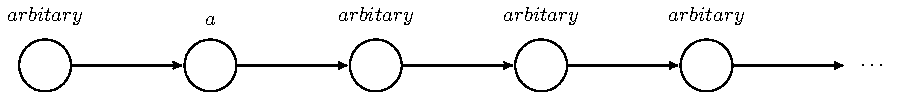
\includegraphics[width=\textwidth]{Img/path_for_Oa.pdf}
    \end{subfigure}
    \\
    \begin{subfigure}{0.8\textwidth}
        \centering
        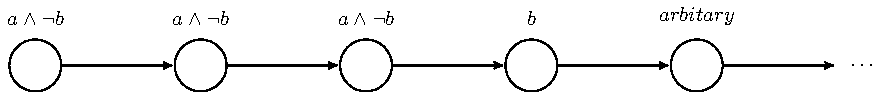
\includegraphics[width=\textwidth]{Img/path_for_aUb.pdf}
    \end{subfigure}
    \caption{路径命题公式$\pi\models O a $与 $\pi\models a U b$的图示}
    \label{fig:path-formula-basic}
\end{figure}
在模型检测中,有三类比较重要的可达性问题,分别是可达性、持续可达性以及重复可达性。过程中主要涉及以下路径命题公式:\(\lozenge\) 表示最终(eventually),\(\square\)表示总是(always),\(\lozenge\square\)表示总是最终(always eventually),\(\square\lozenge\)表示最终总是(eventually always)。其中\(\lozenge\)和\(\square\)具体定义为:
\begin{itemize}
    \item \(\lozenge\varphi\overset{\text{def} }{=} \text{True}U\varphi\)
    \item \(\square\varphi\overset{\text{def} }{=} \neg\lozenge\neg\varphi\)
\end{itemize}
图\ref{fig:path-formula}展示了这两种基本路径命题公式的直观示意图。
\begin{figure}[!htbp]
    \centering
    \begin{subfigure}[b]{0.8\textwidth}
        \centering
        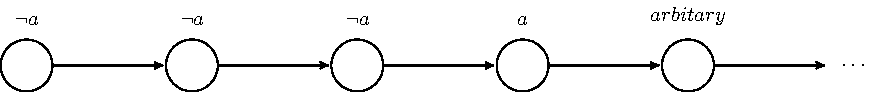
\includegraphics[width=\textwidth]{Img/path_for_Dia.pdf}
    \end{subfigure}
    \\
    \begin{subfigure}{0.8\textwidth}
        \centering
        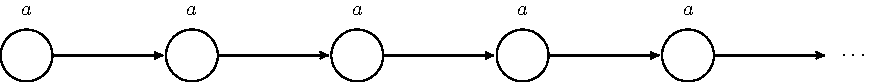
\includegraphics[width=\textwidth]{Img/path_for_SQa.pdf}
    \end{subfigure}
    \caption{路径命题公式$\pi\models\lozenge a$与 $\pi\models\square a$的图示}
    \label{fig:path-formula}
\end{figure}

具体的可满足条件为:
\begin{itemize}
    \item \(\pi\models\lozenge\varphi,iff\exists j\ge0.\pi[j)\models\varphi\)
    \item \(\pi\models\square\varphi,iff\forall j\ge 0.\pi[j)\models\varphi\)
    \item \(\pi\models\lozenge\square\varphi,iff\exists i\ge 0.\forall j\ge i,\pi[j)\models\varphi\)
    \item \(\pi\models\square\lozenge\varphi,iff\forall i\ge 0.\exists j\ge i,\pi[j)\models\varphi\)
\end{itemize}
% //TODO:add some explian
基于此三种可达性问题定义分别如下:
\begin{itemize}
    \item 可达性:\( Pr^{\mathcal{M}}(s \models \lozenge G) = Pr^M(\pi \models \lozenge G : \pi \in \text{Paths}(s))\)
    \item 持续可达性:\( Pr^{\mathcal{M}}(s \models \lozenge \square G) = Pr^M(\pi \models \lozenge \square G : \pi \in \text{Paths}(s))\)
    \item 重复可达性:\( Pr^{\mathcal{M}}(s \models\square \lozenge G) = Pr^M(\pi \models \square\lozenge G : \pi \in \text{Paths}(s))\)
\end{itemize}
\begin{example}
    在例子\ref{ex-transition}中介绍了一个简化版的交通指挥灯的跃迁系统模型。在交通系统中,如果行人可以安全开始穿越,那么在下一个时刻,行人应该继续穿越,直到他们需要停止穿越。这样的命题可以转化为时序命题公式:
    \begin{equation}
        safe \rightarrow O(continue\ U\ stop )
    \end{equation}
    类似地,需要关心行人总能安全地通过路面。这样的命题可以转化为路径命题公式:
    \begin{equation}
        \pi \models \square\lozenge safe
    \end{equation}
\end{example}

\subsection{量子模型检测使用的量子逻辑}
本小节将简单介绍在量子模型中使用的量子逻辑,具体内容可以参考\citep{2021}。
目前量子的模型检测,主要使用Birkhoff-von Neumann Quantum Logic来描述量子系统的性质
% \citep{birkhoff1987logic}
。Birkhoff-von Neumann量子逻辑是一种非经典逻辑,用于描述量子力学中事件的逻辑结构。它由 Birkhoff 和 von Neumann 在 1936 年首次提出。在量子逻辑中,命题的集合不再形成布尔代数,而是形成一个投影算子的正交完备格,这与传统的逻辑系统不同。


\subsubsection*{量子命题}
\label{sec-logic}
在 Birkhoff-von Neumann 量子逻辑中,量子系统的状态可以由希尔伯特空间(Hilbert space)来描述,每个量子命题对应希尔伯特空间的一个闭子空间。对于系统的状态 \(|\psi\rangle\),如果它属于某个特定的闭子空间 \( \mathcal{X} \),可以说这个命题是真的。

\begin{example}\citep{2021}
    考虑以下量子逻辑命题:

\begin{itemize}
\item 命题 \( \mathcal{X} \):在时间 \( t \) 时,量子粒子的位置 \( x \) 坐标在区间 \( [a, b] \) 内。
\item 命题 \( \mathcal{Y} \):在时间 \( t \) 时,量子粒子的动量 \( y \) 坐标在区间 \( [a, b] \) 内。
\end{itemize}
这些命题 \( \mathcal{X} \) 和 \( \mathcal{Y} \) 可以通过粒子的状态希尔伯特空间的特定子空间来表示。
\end{example}


上述将子空间视为原子命题的想法也可以用量子测量来解释。假设系统的一个基本性质由希尔伯特空间$\mathcal{H}$的一个闭子空间$\mathcal{X}$描述。
在量子力学中,为了检查这个性质是否满足,需要对系统当前态$|\psi\rangle$执行一个二元(是或否)测量$\{P_{\mathcal{X}}, P_{\mathcal{X}}^{\perp}\}$,
其中$P_{\mathcal{X}}$和$P_{\mathcal{X}}^\perp$分别是到$\mathcal{X}$和它的正交补$\mathcal{X}^\perp$的投影。测量结果通常是非确定性,其对应概率分别为:
\begin{itemize}
    \item $\mathcal{X}$在$|\psi\rangle$中满足的概率是$\langle\psi|P_{\mathcal{X}}|\psi\rangle$。
    \item 不满足的概率是
    $\langle\psi|P_{\mathcal{X}}^\perp|\psi\rangle = 1 - \langle\psi|P_{\mathcal{X}}|\psi\rangle$。
\end{itemize}
同时可以通过设置一个阈值$\lambda \in [0,1]$来定义关于满足的概率的量化关系:

\begin{definition}\citep{2021}
    如果$\langle\psi|P_{\mathcal{X}}|\psi\rangle \rhd \lambda$,则称$|\psi\rangle$是$(\lambda, \rhd)$满足子空间$\mathcal{X}$描述的命题。其中其中$\rhd \in \{<, \leq, >, \geq\}$。 
\end{definition}

在本文工作的研究中只考虑定性满足,即阈值$\lambda$为0或1时的$(\lambda, \rhd)$满足。显然,对于任何纯态$|\psi\rangle$和子空间$\mathcal{X}$,都有:

\begin{itemize}
\item 如果$|\psi\rangle \in \mathcal{X}$,那么$\mathcal{X}$在$|\psi\rangle$中$(1, \geq)$-满足;
\item 如果$|\psi\rangle \in \mathcal{X}^\perp$,那么$\mathcal{X}$在$|\psi\rangle$中$(0, \leq)$-满足。
\end{itemize}

\subsubsection*{量子逻辑中的连接词}
\label{sec-connect}
在数学上,这种集合的命题逻辑结构可以使用格理论(lattice theory)来描述,其中格中的元素对应于量子事件,格的操作则对应于逻辑运算。在确定了原子命题后,需要引入连接词,这些连接词可以用来构建更复杂的命题,以描述量子系统的复杂属性。在语义上,这些可以被视为在希尔伯特空间$\mathcal{H}$的一个子空间 \(S(\mathcal{H})\) 中的代数操作\citep{2021}。
具体如下:

\begin{itemize}
    \item 子空间之间的包含关系 \( \subseteq \) 在 \(S(\mathcal{H})\) 中是一个偏序关系,它可以理解为量子逻辑的蕴含(元逻辑)。
    \item 一个子空间 \( \mathcal{X} \) 的正交补 \( \mathcal{X}^\perp \) 在量子逻辑中用作否定的解释。
    \item \(S(\mathcal{H})\) 对交集是封闭的,即对于 \(S(\mathcal{H})\) 中的任何元素族 \( \{\mathcal{X}_i\} \),都有$\bigcap_{i} \mathcal{X}_{i} \in \mathcal{S}(\mathcal{H})$。在量子逻辑中用于表示合取。
    \item 对于一组子空间 \(\{\mathcal{X}_i\}\),这些子空间的并定义为
    \(
    \bigvee_i \mathcal{X}_i = \text{span} \left( \bigcup_i \mathcal{X}_i \right).
    \)。在量子逻辑中,析取被解释为子空间的并。
\end{itemize}


量子逻辑中的析取被解释为子空间的并运算。\( (S(\mathcal{H}), \cap, \vee, \perp) \) 构成一个正交模格(orthomodular lattice),\( \subseteq \) 是其序关系,这是 Birkhoff–von Neumann 量子逻辑的代数模型。

在实际应用中,通常只选择$\mathcal{S}(\mathcal{H})$的一个子集$AP$作为原子命题的集合。$AP$的元素可以被看作是真正关注的命题,而其他命题可能是无关的。为了算法的目的,通常假设$AP$是$\mathcal{S}(\mathcal{H})$的一个可列或者甚至是有限的子集,而不是作为原子命题的集合使用$\mathcal{S}(\mathcal{H})$本身,因为$\mathcal{S}(\mathcal{H})$是无穷无尽的。

\subsubsection*{量子逻辑中的满足}
在量子逻辑中,“满足”(satisfaction)意味着量子系统的状态可以在逻辑表达式指定的条件下被视为真。对于任何原子命题$\mathcal{X} \in AP$和状态$|\psi\rangle \in \mathcal{H}$,如果$|\psi\rangle \in \mathcal{X}$,那么说状态$|\psi\rangle$满足$\mathcal{X}$。用$L(|\psi\rangle)$表示在状态$|\psi\rangle$中被满足的原子命题集合:

\begin{equation}
L(|\psi\rangle) = {\mathcal{X} \in AP : |\psi\rangle \in \mathcal{X}}.
\end{equation}

有时,需要在一个状态$|\psi\rangle$和一个不在$AP$中的命题$\mathcal{X}$之间建立更一般的满足关系。例如,在某些应用中,可能对一个命题$\mathcal{X}$是否被一个状态$|\psi\rangle$满足感兴趣,但由于内存的考虑,量子模型检测中一般只会选择了一个非常有限的不包括$\mathcal{X}$的原子命题集合。

对于这样一个不在$AP$中的命题$\mathcal{X}$。给定一个原子命题集合$AP$,其中$\mathcal{X} \in \mathcal{S}(\mathcal{H})$。
如果$\bigcap_{\mathcal{Y} \in L(|\psi\rangle) }\mathcal{Y} \subseteq \mathcal{X}$,那么状态$|\psi\rangle$满足$\mathcal{X}$,记作$|\psi\rangle \models_{AP} \mathcal{X}$或简单地$|\psi\rangle \models \mathcal{X}$。
直观地说,$\bigcap_{\mathcal{Y} \in L(|\psi\rangle)} \mathcal{Y}$是可以用原子命题来定义并描述状态$|\psi\rangle$的最弱陈述。因此,包含关系意味着在状态$|\psi\rangle$中成立的原子命题集合共同蕴含命题$\mathcal{X}$。而如果$\mathcal{X} \in AP$,那么$|\psi\rangle \models \mathcal{X}$当且仅当$|\psi\rangle \in \mathcal{X}$。

\begin{example}\citep{2021}
    % //TODO: rewrite
    设$\mathcal{H}$是一个$n$维希尔伯特空间,它的标准正规基是$\{|0\rangle, |1\rangle, \cdots, |n - 1\rangle\}\ (n \geq 2)$,令$|\psi\rangle = \frac{1}{\sqrt{2}}(|0\rangle + |1\rangle)$。
    \begin{itemize}
        \item 如果取$AP$为与基态$|0\rangle$正交的子空间:

        \begin{equation}
        AP = {\mathcal{Y} \in \mathcal{S}(\mathcal{H}) : |0\rangle \perp \mathcal{Y}},
        \end{equation}
        
        那么$L(|\psi\rangle) = \varnothing$,因此
        
        \begin{equation}
        {\bigcap_{\mathcal{Y} \in L(|\psi\rangle)} \mathcal{Y} = \mathcal{H}.}
        \end{equation}
        
        所以对于任何$\mathcal{X} \in \mathcal{S}(\mathcal{H})$,有$|\psi\rangle \models \mathcal{X}$当且仅当$\mathcal{X} = \mathcal{H}$。
        
        \item 设$AP$为$\mathcal{H}$的2维子空间。对于$n = 2$的情况,
        \begin{equation}
            {\bigcap_{\mathcal{Y} \in L(|\psi\rangle)} \mathcal{Y} = \mathcal{H}}
            \end{equation}
            
            那么有$|\psi\rangle \models \mathcal{X}$当且仅当$\mathcal{X} = \mathcal{H}$。对于$n > 2$的情况,
            
            \begin{equation}
            {\bigcap_{\mathcal{Y} \in L(|\psi\rangle)} \mathcal{Y} = \operatorname{span}\{|\psi\rangle}\}
            \end{equation}
            
            并且$|\psi\rangle \models \mathcal{X}$当且仅当$|\psi\rangle \in \mathcal{X}$。
            
        \item 如果$AP$是包含基态$|2\rangle$的子空间,即$AP = \{\mathcal{X} \in \mathcal{S}(\mathcal{H}) : |2\rangle \in \mathcal{X}\}$,那么
            
            \begin{equation}
            {\bigcap_{\mathcal{Y} \in L(|\psi\rangle)} \mathcal{Y} = \operatorname{span}\{|\psi\rangle, |2\rangle}\}
            \end{equation}
            
            并且$|\psi\rangle \models \mathcal{X}$当且仅当$|\psi\rangle,|2\rangle \in \mathcal{X}$。
    \end{itemize}

\end{example}
\section{TDD简介}
TDD是一种决策图样式的数据结构,用于使用张量网络表示量子线路。
本节将从用张量网络表示量子线路开始,简单介绍张量网络如何转换到TDD,最后简单介绍TDD与类似表示的对比。
有关TDD的具体内容,可以参考\citep{Hong_2022}。
% 目前,TDD研究集中在开发更有效的算法来使用TDD操作和收缩张量网络。这包括开发新技术来分割张量网络,优化TDD结构,从而进一步提高基于TDD的可达性分析和模型检测算法的效率。这也是实现基于TDD的量子模型检测的主要方法。
\subsection{TDD定义}
张量是与一组与索引序列\(I=\{x_1,\ldots,x_n\}\)相关联的多维线性映射。在量子计算中,可以假设只从\(\{0,1\}\)中取值。因此,张量定义为定义\ref{df-tensor}所示。
\begin{definition}\citep{biamonte2019lectures}
    \label{df-tensor}
    当张量只从从\(\{0,1\}\)中取值时,对于定义在索引序列\(I\)上的张量\(\phi\),其可以表示为一个字典
    \begin{align}
        \phi :{\{0,1\}}^I\rightarrow\mathbb{C}
    \end{align}
    其中\(\mathbb{C}\)为复数。
\end{definition}


因此一个向量表示为$[\alpha_0,\alpha_1]$的量子比特$x$可以描述为秩为$1$的张量$\phi_x$,其中$\phi_x\left(0\right)=\alpha_0, \phi_x\left(1\right)=\alpha_1$。具有输入比特$x$和输出比特$y$的单比特门可以表示为秩为$2$的张量$\phi_{xy}$。类似的$n$比特量子门可以表示成一个秩为$2n$的张量。在张量表示中,一般不区分输入和输出索引。只有当将张量解释为门或线路时会规定关于其信息。

张量之间最重要的运算之一是收缩(contraction)。收缩是通过对共享索引求和获得新的张量。具体来说,设 张量$\gamma_{\overrightarrow{x},\overrightarrow{z}}$ 和 $\xi_{\overrightarrow{y},\overrightarrow{z}}$ 的共享索引集 是$\overrightarrow{z}$。设收缩后的新张量为 $\phi_{\overrightarrow{x},\overrightarrow{y}}$,则其表达式如式子\ref{eq-contraction}所示。
\begin{equation}
\label{eq-contraction}
\phi_{\overrightarrow{x},\overrightarrow{y}}(\overrightarrow{a},\overrightarrow{b}) = \sum_{\overrightarrow{c} \in \{0,1\}^{\overrightarrow{z}}} \gamma_{\overrightarrow{x},\overrightarrow{z}}(\overrightarrow{a}, \overrightarrow{c}) \cdot \xi_{\overrightarrow{y},\overrightarrow{z}}(\overrightarrow{b}, \overrightarrow{c}).
\end{equation}

另一个重要的张量操作是切片(slicing),它对应于布尔函数的余因子运算。设 $\phi$ 是索引序列为 $I$ 上的张量。任取一个索引\(x\in I\),对 $\phi$ 进行关于 $x = c$ 与 $c \in \{0, 1\}$ 的切片也是一个张量 $\phi|_{x=c}$,在索引集 $I' =I/\{x\}$ 上定义如式子\ref{eq-slicing}所示。
\begin{equation}
    \label{eq-slicing}
\phi|_{x=c}(\overrightarrow{a}) := \phi(c, \overrightarrow{a})
\end{equation}
对于任意 $\overrightarrow{a} \in \{0, 1\}^n$。称 $\phi|_{x=0}$ 和 $\phi|_{x=1}$ 分别为 $\phi$ 关于 $x$ 的负切片(negative slicing)和正切片(positive slicing)。如果 $\phi|_{x=0} \neq \phi|_{x=1}$,称索引 $x \in I$ 对于 $\phi$ 是本质的(essential)。
% 同时张量满足定理\ref{lemma-tensor}中的性质。

% \begin{lemma}
%     \label{lemma-tensor}
%     对于定义在索引序列\(I\)上的张量\(\phi\),其中的每个索引\(x\in I\),都有
%     \begin{align}
%         \phi = \bar{x}\cdot \phi|_{x=0}+x\cdot \phi|_{x=1}
%     \end{align}
% \end{lemma}

张量网络是一个无向图\(G=\left(V,E\right)\)。其中顶点集$V$中的每个顶点$v$表示一个张量。边集\(E\)中每条边\(e\)代表与相邻两个张量相关联的公共索引。通过以任意顺序收缩连接的张量,可以得到一个秩为\(m\)的张量,其中\(m\)是$G$中开放边数。这个独立于收缩顺序的张量也称为该张量网络的张量表示\citep{biamonte2019lectures}。
张量网络提供了一种新的量子线路表示方法\citep{pednault2017breaking}。而当给定量子线路中所有量子门的输入和输出状态的索引值,收缩掉共享的索引,就可以得到量子线路的张量表示。


TDD是一种具有决策图和张量网络特征的数据结构\citep{Hong_2022}。它可用于表示张量,并进一步表示量子线路。与BDD(Boolean Decision Diagrams)类似,TDD是一种建立在索引顺序$I=\{x_1,\ldots,x_n\}$上的决策树模型。具体定义定义\ref{df-tdd}所示。
\begin{definition}\citep{Hong_2022}
    \label{df-tdd}
    TDD是一个建立在索引顺序$I=\{x_1,\ldots,x_n\}$上的有根节点,带权重的有向无环图,其中包括:
    \begin{align}
        \mathcal{F}=\left(V,E,index,value,low,high,w\right)
    \end{align}
    其中:
    \begin{enumerate}
        \item $V$是一个有限节点集,被划分为非终端节点$V_n$和终端节点$V_T$。用$r_{\mathcal{F}}$表示$\mathcal{F}$的唯一根节点。
        \item $E=\left\{\left(v,low\left(v\right)\right),\left(v,high\left(v\right)\right):v\in V_N\right\}$是树中所有边集合,其中$\left(v,low\left(v\right)\right)$和$\left(v,high\left(v\right)\right)$分别称为v的低边和高边,分别指向该节点索引的负切片和正切片。根结点$r_{\mathcal{F}}$具有唯一的入射边$e_{\mathcal{F}}$,该入射边没有源结点。
        \item $index:V_r\rightarrow I$将每个非终端节点分配给I中的索引。
        \item $value:V_T\rightarrow\mathbb{C}$将每个终端节点赋予一个复数值。
        \item $low$和$high$都是$V_N\rightarrow V$中的映射,它们分别为每个非终端节点指定其低边和高边后继。
        \item $w:E\rightarrow\mathbb{C}$将每条边赋予一个复数权重。特别地,$w\left(e_r\right)$称为$\mathcal{F}$的权重,并记作$w_{\mathcal{F}}$。
    \end{enumerate} 
\end{definition}


对于TDD中的一个节点$v$,如果$v$是终端节点,则$\phi\left(v\right):= value (v)$是一个秩为$0$的张量,即常数,也可以称为一个平凡TDD。如果$v$是非终端节点,则根据定义,该节点表示的张量如式子\ref{eq-non-term}所示。
\begin{align}
    \label{eq-non-term}
    \phi(v):=w_{0} \cdot \overline{x_{v}} \cdot \phi(\operatorname{low}(v))+w_{1} \cdot x_{v} \cdot \phi(h i g h(v))
\end{align}
其中$x_v=index\left(v\right),\overline{x_{v}}=1-index\left(v\right)$。而整个TDD也可以表示为:
\begin{align}
    \phi\left(\mathcal{F}\right)=w_{\mathcal{F}}\cdot\phi\left(r_{\mathcal{F}}\right)
\end{align}


% \subsection*{TDD的规范与化简}
\label{sec-reduce}
根据定义得到的TDD在结构上显然比较冗余,可以进行进一步化简。具体过程是先进行规范化(normalized),让后进行化简(reduced)\citep{Hong_2022}。
其中规范化的目的是使得TDD的终端节点只包含0和1,同时将终端节点的张量值沿路径逐步上移。具体规范步骤如下:
\begin{enumerate}
    \item 如果$v$是一个非零值$value\left(v\right)\neq 1$的终端节点,则将其值设置为1,并将每个入边的权重w更改为$value\left(v\right)\cdot w$。\label{norm1}
    \item 假设v是一个非终端节点,且$\phi\left(v\right)\neq 0$。首先规范化$\phi\left.\left(low(v\right)\right)$和$\phi\left.\left(high(v\right)\right)$。完成$\phi\left.\left(low(v\right)\right)$和$\phi\left.\left(high(v\right)\right)$的规范化后。如果$\phi\left.\left(low(v\right)\right)\neq 0$,并且此时$\phi\left.\left(high(v\right)\right)=0$或$\left|w_0\right|\geq\left|w_1\right|$,则将$w$设置为$w_0$。否则,将$w$设置为$w_1$。然后更新$w_0≔w_0/w,w_1≔w_1/w$。此时完成$v$的规范化。\label{norm2}
\end{enumerate}



在完成规范化后,此时的TDD终端节点只包含0和1。可以进一步简化TDD,使得TDD只包含一个终端节点1,同时尽量使用重复出现的张量。具体简化步骤如下:
\begin{enumerate}
    \item 	合并所有值为1的终端节点。删除所有终端$0$节点,并将它们的入边重定向到唯一的终端节点,并将它们的权重重置为$0$。\label{sympl1}
	\item 将所有权重为$0$的边重定向到终端节点。如果根节点的入边权重为$0$,则终端节点成为新的根,该TDD为空。删除所有从根节点不可达的节点,以及涉及它们的所有边。\label{sympl2}
	\item 如果一个节点v的低边和高边后继相同,并且其低边和高边具有相同的权重w,则删除该节点。如果入边权重$w=0$,则将其传入边重定向到终端节点。否则,将其传入边重定向到其后继节点。\label{sympl3}
	\item 合并两个具有相同索引、相同$0$和$1$后继以及对应边上相同权重的节点。\label{sympl4}
\end{enumerate}


为了阅读简洁,下文中无特殊说明的TDD均指化简后的TDD,即reduced tensor decision diagrams。
% 结合以上步骤,算法\ref{alg-tdd}简单展示了如何将给定的张量\(\phi\)转换为对应的TDD表示。
% \begin{algorithm}
%     \caption{生成张量\(\phi\)的TDD表示TDD(\(\phi\))\citep{Hong_2022}}
%     \label{alg-tdd}
%     \begin{algorithmic}[1]
%     \Require 一个张量\(\phi\) 和对应的索引顺序\(I\)
%     \Ensure \(\phi\)的TDD表示TDD(\(\phi\))
%     \If{\(\phi = c\),即输入张量是一个标量}
%         \State \Return 带权重$c$的平凡TDD
%     \EndIf
%     \State \(x \gets\) \(\phi\)在索引顺序\(I\)中最小的索引
%     \State \(tdd \gets\) 一个空的TDD
%     \State \(tdd.root \gets\) 一个索引为\(x\)的新节点\(v\) 
%     \State \(v.low \gets\) 递归调用本算法,得到\(\phi|_{x=0}\)对应的TDD表示TDD(\(\phi|_{x=0}\))
%     \State \(v.high \gets\) 递归调用本算法,得到\(\phi|_{x=1}\)对应的TDD表示TDD(\(\phi|_{x=1}\))
%     \State \(tdd.weight \gets 1\)
%     \State \Return \(tdd\)化简后的TDD表示
%     \end{algorithmic}
% \end{algorithm}


\subsection{TDD与类似表示}
\label{sec-compare}
TDD是一种相对较新的数据结构,用于表示和操作张量网络。与之类似的表示方法有张量网络TN和量子多值决策图QMDD。本节的最后将讨论定义\ref{df-tensor}中的张量网络TN,定义\ref{df-tdd}中的张量决策图TDD,以及QMDD\citep{1623982}三种表示的效率。

张量网络TN提供了量子线路更紧凑的表现形式。但在张量之间的收缩过程中,如式子\ref{eq-contraction}所示,张量网络需要对要收缩的索引进行大量的加法操作。而TDD基于决策数的结构可以借助树算法,减少加法运算,从而快速得到收缩结果。
因此TDD表示量子线路,一般会比TN节省更多资源。

QMDD(Quantum Multiple-Valued Decision Diagrams),即量子多值决策图提供了一种紧凑而系统的方法来描述量子过程。目前QMDD已有效地用于量子线路的合成\citep{niemann2020advanced}和和验证任务
\citep{burgholzer2020verifying,burgholzer2020advanced}。
图\ref{fig:qmdd-basic}展示了一个矩阵到最终QMDD的一个过程。
\begin{figure}[htbp]
    \centering
    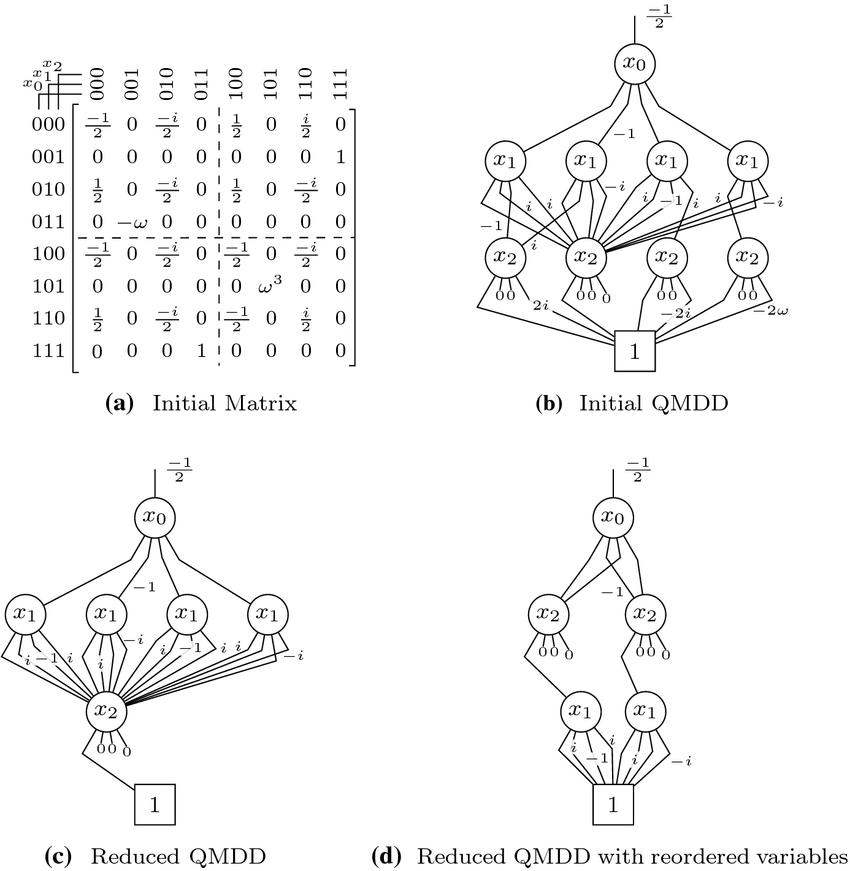
\includegraphics[height=10cm]{Img/QMDD-intro}
    \caption{从矩阵到QMDD的示例\citep{1623982}}
    \label{fig:qmdd-basic}
\end{figure}

可以看到QMDD和TDD的相似点有:
\begin{enumerate}
    \item 二者都存在唯一的终端顶点,值为1。该终端顶点没有出边。
    \item 二者都有唯一一个顶点作为起始顶点,它有一个单独的入边,该入边本身没有源顶点。
    \item 二者中的每条边(包括指向起始顶点的边)都有一个关联的复数值权重。
    \item 二者中的索引都按一定顺序排列,并且都满足以下两条规则:
    \begin{enumerate}[label=\roman*)]
        \item 每个索引在从起始顶点到终端顶点的每条路径上最多出现一次。
        \item 来自索引排序低的非终端顶点的边指向索引排序高的非终端顶点或终端顶点。
    \end{enumerate}
    \item 二者都尽量复用节点,即没有两个标记索引相同的非终端顶点有相同的出边集(即连接节点和边权重都一致)。
\end{enumerate}

QMDD和TDD主要不同的在于QMDD结构中,每个非终端节点连接有四个后继节点。
而在TDD结构中,每一个非终端节点分别连接着两个后继节点。
因此从原理上讲,如果采用相同的排序规则,量子线路的TDD表达方式的节点数大约是其QMDD表达方式节点数的两倍。但由于它们都拥有相同数目的加权边并记录了相同数量的权值(即复数)。此时TDD表达方式所需的内存空间与QMDD表达方式所需的内存空间持平。

虽然TDD的表示形式和QMDD紧凑程度相近。
但是TDD非常灵活,可以轻松与张量网络中的一些优化技术结合以进一步提高其表现。

综上,TDD的效率一般比TN的表示效率高,与QMDD类似。但TDD的高度灵活性,使得TDD的发展可能比QMDD更好。特别地,\cite{Hong_2022}中进行了三者的数值对比实验,验证了TDD的表示优势。
这是本次研究中选择TDD作为表示线路的最重要原因。
% 图\ref{fig:tdd-compare}是\cite{Hong_2022}中展示的目前各种比较成熟的表示方法下模拟量子线路的时间对比。其中TDD No Part指的是不对线路进行拆分优化的方法。TDD part I 和TDD part II是两种的张量网络中的优化技术。
% QMDD指的是Quantum Multiple-valued Decision Diagrams。
% TN表示方法使用了google的tensor network\citep{roberts2019tensornetwork}。
% 从图\ref{fig:tdd-compare}可以看到,两种TDD的优化方案都是时间消耗最少的。不使用拆分优化的TDD No Part与QMDD时间接近。而当比特数少于10时,TN的时间少于TDD No Part,但随着比特数增加,TN的用时快速超过TDD No Part。
% 因此TDD相比其他表示方式有一定优势。这是本文工作研究中选择TDD作为主要技术的重要原因。

% \begin{figure}[!htbp]
%     \centering
%     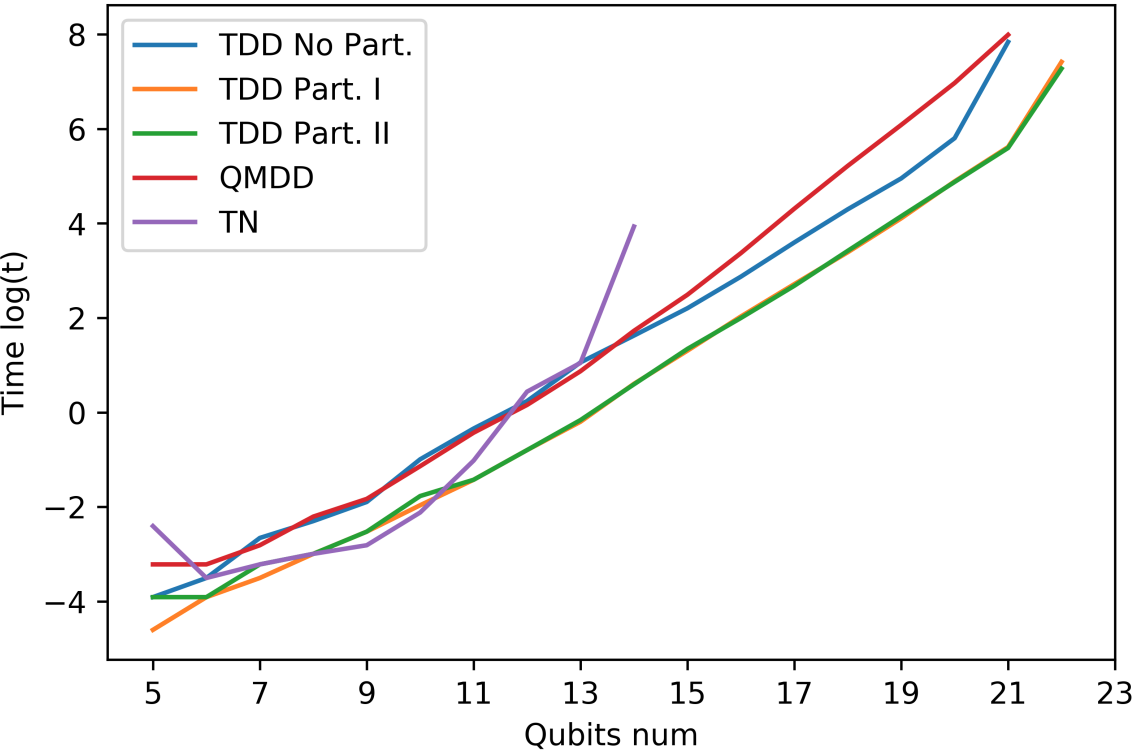
\includegraphics[height=8cm]{Img/tdd-compare.pdf}
%     \caption{对QFT线路,TDD与TN,QMDD表示的比较\citep{Hong_2022}}
%     \label{fig:tdd-compare}
% \end{figure}

\section{本章小结}
本章主要介绍了本文工作的研究的相关背景知识,包括量子计算,模型检测和TDD的基础理论。

第一部分介绍了量子计算的相关知识,包括量子力学基本原理、量子线路模型等。量子力学建立在希尔伯特空间、算符等数学基础之上,描述了量子系统的状态、演化和测量。量子线路则是一种描述量子计算的模型,通过对量子比特进行初始化、施加量子门操作和测量等来执行量子计算任务。

第二部分介绍了模型检测的基础知识,包括跃迁系统、时序逻辑和量子模型检测。跃迁系统用于对待检测系统建模,定义了系统状态、行为及状态转移关系。时序逻辑用于指定待验证的属性,讨论了状态命题和路径命题等。量子模型检测则利用Birkhoff-von Neumann量子逻辑描述量子系统的性质,阐述了量子逻辑中命题的表示、逻辑结构及满足关系等。

第三部分从张量网络出发,介绍了TDD的相关定义。TDD是基于量子张量网络的表示方法。因此这部分从张量网络表示量子线路的方法开始。然后,对TDD数据结构进行了简单定义。
随后,本章详细介绍了如何将张量网络转换为TDD表示,包括TDD的规范化和化简策略。
为了全面理解TDD的实际效果,将其与QMDD和张量网络的表示方法进行了简单讨论,分析了TDD的优势。

本章的背景知识为后续开展基于TDD的量子模型检测研究奠定了理论基础。
% 本章最后指出,通过张量网络表示量子线路和量子系统,并借助张量决策图进行量子模型检测是本文工作的研究的主要目标。

% 总的来说,本章对量子计算、模型检测及相关数学基础进行了概括性介绍,为读者了解本文的内容做好了铺垫。